\input{../../.preambles/01-semester_work}
\input{../../.preambles/10-russian}
\input{../../.preambles/20-math}
\input{../../.preambles/30-physics}

\begin{document}

\maketitlepagewithvariant{Факультет электроники и вычислительной техники}
{<<Высшая математика>>}{Теория вероятности}{студент группы Ф-369\\Голубев~А.~В.}
{Шушков~В.~И.}{№1}{6}

\newpage

\emph{1. Какова вероятность того, что случайно составленное трёхзначное число 
не содержит цифры 2? }

\emph{Решение:}

Используем классическую формула для подсчёта вероятности:
\[ P = \frac{m}{n} \]
В роли \( m \) будет играть размещение трёх чисел из десяти возможных:
\[ 
	m = A^{3}_{10} = \frac{10!}{(10-3)!} = 
	\frac{10\cdot9\cdot8\cdot7!}{7!} = 720 
\]
В место \( n \) общее количество чисел, то есть \( n = 1000 \). В итоге 
получаем
\[ P = \frac{720}{1000} = 0.72 \]

\emph{Ответ: } \( P = 0.72 \) \\\\

%------------------------------------------------------------------------------

\emph{2. Имеется семь карточек разрезной азбуки с буквами <<С>>, <<Е>>, <<М>>, 
<<Е>>, <<С>>, <<Т>>, <<Р>>. Карточки тщательно перемешиваются. Какова 
вероятность того, что при последовательном извлечении всех карточек 
получится слово <<семестр>> ?}

\emph{Решение:}

На карточках имеются две буква <<С>>, две <<Е>> и остальных букв по одной. 
Поэтому, первая буква слова <<семестр>> может быть выбрана двумя способами, 
вторая двумя способами, а остальные буквы могут быть выбраны только одним 
способом. Таким образом, число \( m \) будет равно произведению этих чисел, 
а число \( n \) количеству перестановок. В итого получаем:
\[ 	
	P = \frac{ 4 }{ 7! } 
	= \frac{ 4 }{ 7\cdot6\cdot5\cdot4\cdot3\cdot2\cdot1 }
	\approx 0.794\cdot10^{-3}
\]

\emph{Ответ: } \( P \approx 0.794\cdot10^{-3} \) 

\newpage

%------------------------------------------------------------------------------

\emph{3. Судно, имеющее одно рулевое устройство, четыре котла и две турбины, 
считается управляемым, если исправно рулевое устройство, хотя бы один из 
котлов и хотя бы одна из турбин. Событие \( A \) означает исправность 
рулевого устройства, \( B_k (k = 1, 2, 3, 4) \) -- исправность \( k \)-го 
котла и \( G_j (j = 1, 2) \) -- исправность \( j \)-ой турбины.}

\emph{Выразить через \( A, B_k \) и \( G_j \) событие \( D \) -- судно является 
управляемым.}

\emph{Решение:}

Представим результирующее событие в виде диаграммы:

\begin{figure}[h!]
        \center
        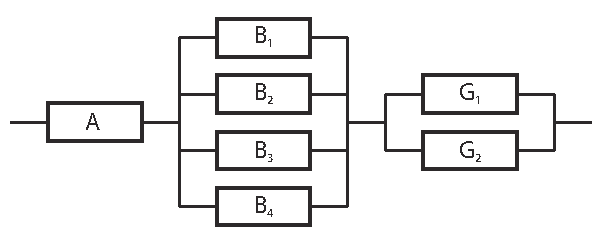
\includegraphics[width=.6\textwidth]{graph}
\end{figure}

Тогда событие \( D \) представимо в виде:

\[ 
	D = A\cdot\left( B_1 + B_2 + B_3 + B_4 \right)\cdot\left( G_1 + G_2 \right) 
\]

\emph{Ответ: } 
\(
	D = A\cdot\left( B_1 + B_2 + B_3 + B_4 \right)\cdot\left( G_1 + G_2 \right) 
\) \\\\

%------------------------------------------------------------------------------

\emph{4. При выборочной проверке партии изделий вероятность отобрать одно 
нестандартное изделие равно \( 0.05 \). Какова вероятность того, что все 
три выбранные наугад изделия окажутся стандартными.}

\emph{Решение:}

Для решения задачи используем формулу Бернулли:
\[ 
	P(n, k) = C^{k}_{n} \cdot p^k \cdot q^{n-k}, \text{ где } q = 1 - p 
\]
Рассматривая текущий случай: \( n = 3, k = 0, p = 0.05 \), где 
\( n \) -- количество выбранных деталей, \( k \) -- количество 
нестандартных и \( p \) -- вероятность выбрать нестандартную. 
Тогда решение представимо в виде:
\[ 
	P(3, 0) = C^{0}_{3} \cdot 1 \cdot q^{3} = 
	\frac{ 3! }{ 0! \cdot 3! } \cdot (1 - 0.05)^3 \approx 0.857
\]

\emph{Ответ: } \( P \approx 0.857 \)

\newpage

%------------------------------------------------------------------------------

\emph{5. Абонент забыл последнюю цифру номера телефона и набирает её 
наудачу. Найти вероятность того, что ему придётся сделать не более двух 
неудачных попыток.}

\emph{Решение:}
\( A \) -- звонок не более двух неудачных попыток.

\( A_1 \) -- цифра, выбранная при первом наборе.

\( A_2 \) -- при втором наборе.

\( A_3 \) -- при третьем наборе.

Тогда вероятность получается:
\[ 
	P(A) = A_1 + A_1 \cdot A_2 + A_1 \cdot A_2 \cdot A_3 
\]
\[ 
	P(A) = P(A_1) + P(A_1 \cdot A_2) + P(A_1 \cdot A_2 \cdot A_3) = 
	\frac{1}{10} + \frac{9}{10}\cdot\frac{1}{9} + 
	\frac{9}{10}\cdot\frac{8}{9}\cdot\frac{1}{8} = 
	\frac{1}{10} + \frac{9}{90} + \frac{72}{720} = 0.3
\]

\emph{Ответ: } \( P = 0.3 \) \\\\

%------------------------------------------------------------------------------

\emph{6. На вход устройства с вероятностью \( 0.8 \) поступает смесь 
полезного сигнала с помехами, а с вероятностью \( 0.2 \) только помеха. 
Если поступает полезный сигнал с помехой, то устройство регистрирует 
наличие какого-то сигнала с вероятностью \( 0.7 \); если только помеха, то 
с вероятностью \( 0.3 \). Известно, что устройство зарегистрировало наличие 
какого-то сигнала. Найти вероятность того, что в его составе есть полезный 
сигнал.}

\emph{Решение:}

Сделаем обозначения \( P_1 = 0.8 \), \( P_2 = 0.2 \), \( P_3 = 0.7 \) и 
\( P_4 = 0.3 \). \\
\emph{Событие A:} есть полезный сигнал \( P(A) = P_1 \) \\
\emph{Событие B:} зарегистрирован сигнал 
\( P(B) = P_1 \cdot P_3 + P_2 \cdot P_4 \)

Используем формулу Байеса
\[ 
	P(A|B) = \frac{P(B|A)\cdot P(A)}{P(B)}
\]
получим вероятность обнаружить полезный сигнал.
\[ 
	P = \frac{P_1 \cdot P_3}{ P_1 \cdot P_3 + P_2 \cdot P_4} 
	= \frac{ 0.8 \cdot 0.7 }{ 0.8 \cdot 0.7 + 0.2 \cdot 0.3}
	\approx 0.903
\]
\emph{Ответ: } \( P \approx 0.903 \)

\newpage

%------------------------------------------------------------------------------

\emph{7. Среди выпускаемой цехом продукции \( 10\% \) является браком. На 
испытании поступила партия из \( 10 \) деталей. Каково наивероятнейшее число 
бракованных деталей в рассматриваемой выборке и какова его вероятность?}

\emph{Решение:}

Так как количество бракованных деталей выпускаемых цехом составляет 
\( 10\% \), то наивероятнейшее число \( m = 1 \). Для нахождения этой 
вероятности воспользуемся формулой Бернулли:
\[
	P(10, 1) = C^{1}_{10} \cdot p \cdot q^{9} = 
	10 \cdot 0.1 \cdot ( 1 - 0.1 )^{9} \approx 0.387
\]

\emph{Ответ: } \( m = 1, P \approx 0.387 \) \\\\

%------------------------------------------------------------------------------

\end{document}